\documentclass[DM,lsstdraft,SDP]{lsstdoc}
%Replace the CUx here and all \CU will resolve below.

\usepackage{gwp}
\usepackage{risk}
\usepackage{longtable}

\begin{document}

\setDocTitle    [Development Plan \CU]
                    {\color[rgb]{0.16,0.42,0.57} \sf \CU  ~Software
                    Development Plan}
\setDocAuthor   {theAuthor}                % the author(s)
\setDocApprove  {LSST Project Office}              % approval by ...
\setDocRef      {LDM-NUM} % the reference code
\setDocIssue    {0D}                        % the issue
\setDocRevision {1}                        % the revision
\setDocDate     {\today}              % the date of the issue
\setDocStatus   {draft}                    % the document status

%
% a short abstract
%
\setDocAbstract {This is a template for a Gaia DPAC Software
   Development Plan for \CU. It outlines the development approach,
   management structure, work breakdown, configuration control etc.
   for the development of the \CU software.}

%
% the title page
%
\mktitle

%
%   Revision history
%
% MOST RECENT FIRST
\begin{docHistory}
\addtohist{D}{1}{yyyy-mm-dd}{myInitials}{First draft}
\end{docHistory}

%
%   TOC
%
\newpage
\setcounter{tocdepth}{3}
\tableofcontents
\newpage

%
% It's all yours from here on
%

\section{Introduction \label{sect:intro}}
\subsection{Scope \label{sect:scope}}
This document covers all development in \CU.

\subsection{Applicable Documents \label{sect:appdocs}}
\begin{tabular}[htb]{l l}
\citell{LL:WOM-017}& Project Implementation Plan for Gaia DPAC\\
\citell{LL:RD-010}& Gaia DPAC Project Development Plan\\
\citell{LL:WOM-001}& Work Breakdown Structures for Gaia DPAC\\
\citell{LL:TL-001}&       DPAC Product Assurance Plan \\
\citell{LL:WOM-012}&      DPAC Software Configuration Management Plan \\
\citell{LL:MP-011}& Document Reference Codes for Gaia \\
\citell{LL:RD-008} & DPAC Risk Management Plan \\
\citell{LL:TLO-001} & ECSS Tailoring \\
\citell{LL:RG-004}  & DPAC System Validation and Test Plan\\
\end{tabular}

\subsection{References\label{sect:references}}
\vspace*{-1cm}
\renewcommand{\refname}{}
\bibliographystyle{gaia_aa}
\bibliography{gaia_livelink_valid,gaia_drafts,gaia_refs,gaia_books,gaia_refs_ads}

\subsection{Acronyms}
The following table has been generated from the on-line Gaia acronym list:
\newline\newline%decrement table counter so table sin doc start at 1.
\addtocounter{table}{-1}
\begin{longtable}{|l|p{0.8\textwidth}|}\hline 
\textbf{Acronym} & \textbf{Description}  \\\hline
API&Application Programming Interface \\\hline
CU&Coordination Unit (in DPAC) \\\hline
DM&Data Management (LSST) \\\hline
DPAC&Data Processing and Analysis Consortium \\\hline
DPACE&Data Processing and Analysis Consortium Executive \\\hline
ECSS&European Cooperation for Space Standardisation \\\hline
ESA&European Space Agency \\\hline
ESAC&European Space Astronomy Centre (VilSpa) \\\hline
ESF&European Science Foundation \\\hline
ESTEC&European Space research and TEchnology Centre (ESA) \\\hline
FOP&Flight Operation Procedure (Plan) \\\hline
GIS&(Astrometric) Global Iterative Solution \\\hline
IOA&Institute of Astronomy (Cambridge; also denoted IOA) \\\hline
LDAP&Lightweight Directory Access Protocol \\\hline
LSST&Large Synoptic Surrvey Telescope \\\hline
LTD&LSST the Docs \\\hline
LaTeX&(Leslie) Lamport TeX (document markup language and document preparation system) \\\hline
MDB&Main Database \\\hline
MOC&Mission Operations Centre \\\hline
NASA&National Aeronautics and Space Administration (USA) \\\hline
PR&Progress Report \\\hline
QA&Quality Assurance \\\hline
SDSS&Sloan Digital Sky Survey \\\hline
SOC&Science Operations Centre \\\hline
SVN&SubVersioN \\\hline
TOC&Table of Contents \\\hline
USA&United States of America \\\hline
WP&Work Package \\\hline
XMM&X-ray Multi-mirror Mission (ESA; officially known as XMM-Newton) \\\hline
\end{longtable} 
 % generated by the acronyms.csh (GaiaTools)

\section{\CU ~role and structure \label{sect:roleandstruct}}

\subsection{Role of  \CU  \label{sect:role}}

\subsection{Organisation and members  \label{sect:org}}
The key functions of \CU{} are the following:
\begin{center}
\begin{longtable}{|m{.25\textwidth}|m{.2\textwidth}|m{.4\textwidth}|}\hline
{\bf Position} & {\bf Name} & {\bf Description} \\\hline
\CU{} Leader &
(Insert Name here) &
\citell{LL:RD-010} (Section A.2.1)
\\\hline
\CU{} Technical Manager &
(Insert Name here) &
\citell{LL:RD-010} (Section A.2.2)
\\\hline
Configuration Manager &
(Insert Name here) &
\citell{LL:WOM-012} (Section 3.1)
\\\hline
Quality Assurance Leader &
(Insert Name here) &
\citell{LL:TL-001} (Section 4)
\\\hline
Risk Manager &
(Insert Name here) &
\citell{LL:RD-008} (Section 5)
\\\hline
Test Manager &
(Insert Name here) &
\citell{LL:RG-004} (Test Personnel sections)
\\\hline
\end{longtable}
\end{center}

This may include an organigram as in \figref{fig:orgdiag}.

  \begin{figure}[htbp]
  \begin{center}
    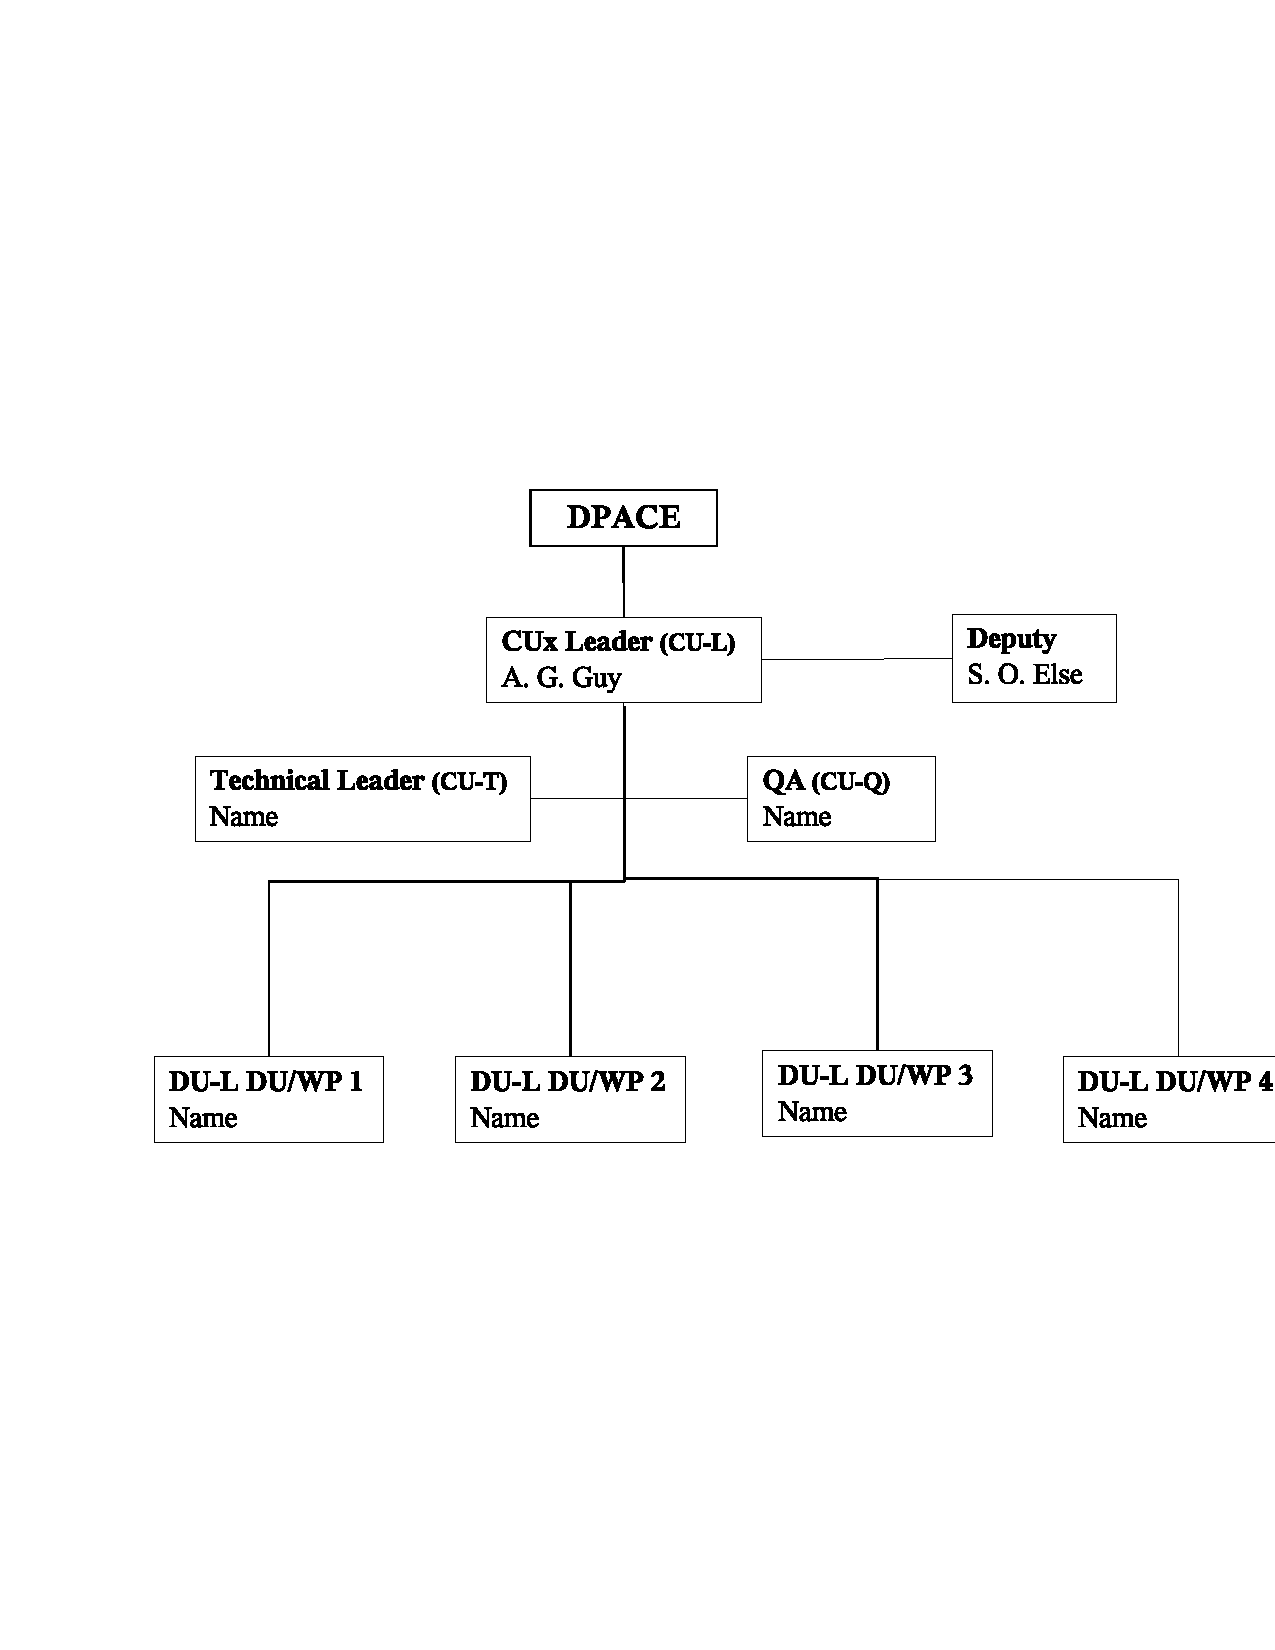
\includegraphics[scale=0.5,trim=0 6cm 0 0]{images/organigram}
      \caption{Example generic organigram for a CU  \label{fig:orgdiag}}
  \end{center}

   \end{figure}

The current number of active members in the CU is around XX though
it might fluctuate slightly in time. For a full list of members use
the Gaia People finder and select the Group \CU. Here is a
convenient link to the list (one must be logged in to the Gaia
portal first)
\url{http://www.rssd.esa.int//SYS/include/people_search_open.php?project=GAIA&action=Retrieve&group_select=gaiaperson.\CU}


\subsection{Product Breakdown Structure\label{sect:decomp}}

In the section the products of \CU ~are outlined. In general for Gaia a
product is related to a top level work package, and may be include SW systems, data and documentation. All top-level SW systems which will have an SRS should be listed (minimum detail), and the Science Products to be produced by the CU should be included A version of the CU1 product tree is included as an example in \figref{fig:prod}.

\begin{figure}[htbp]
\begin{center}
 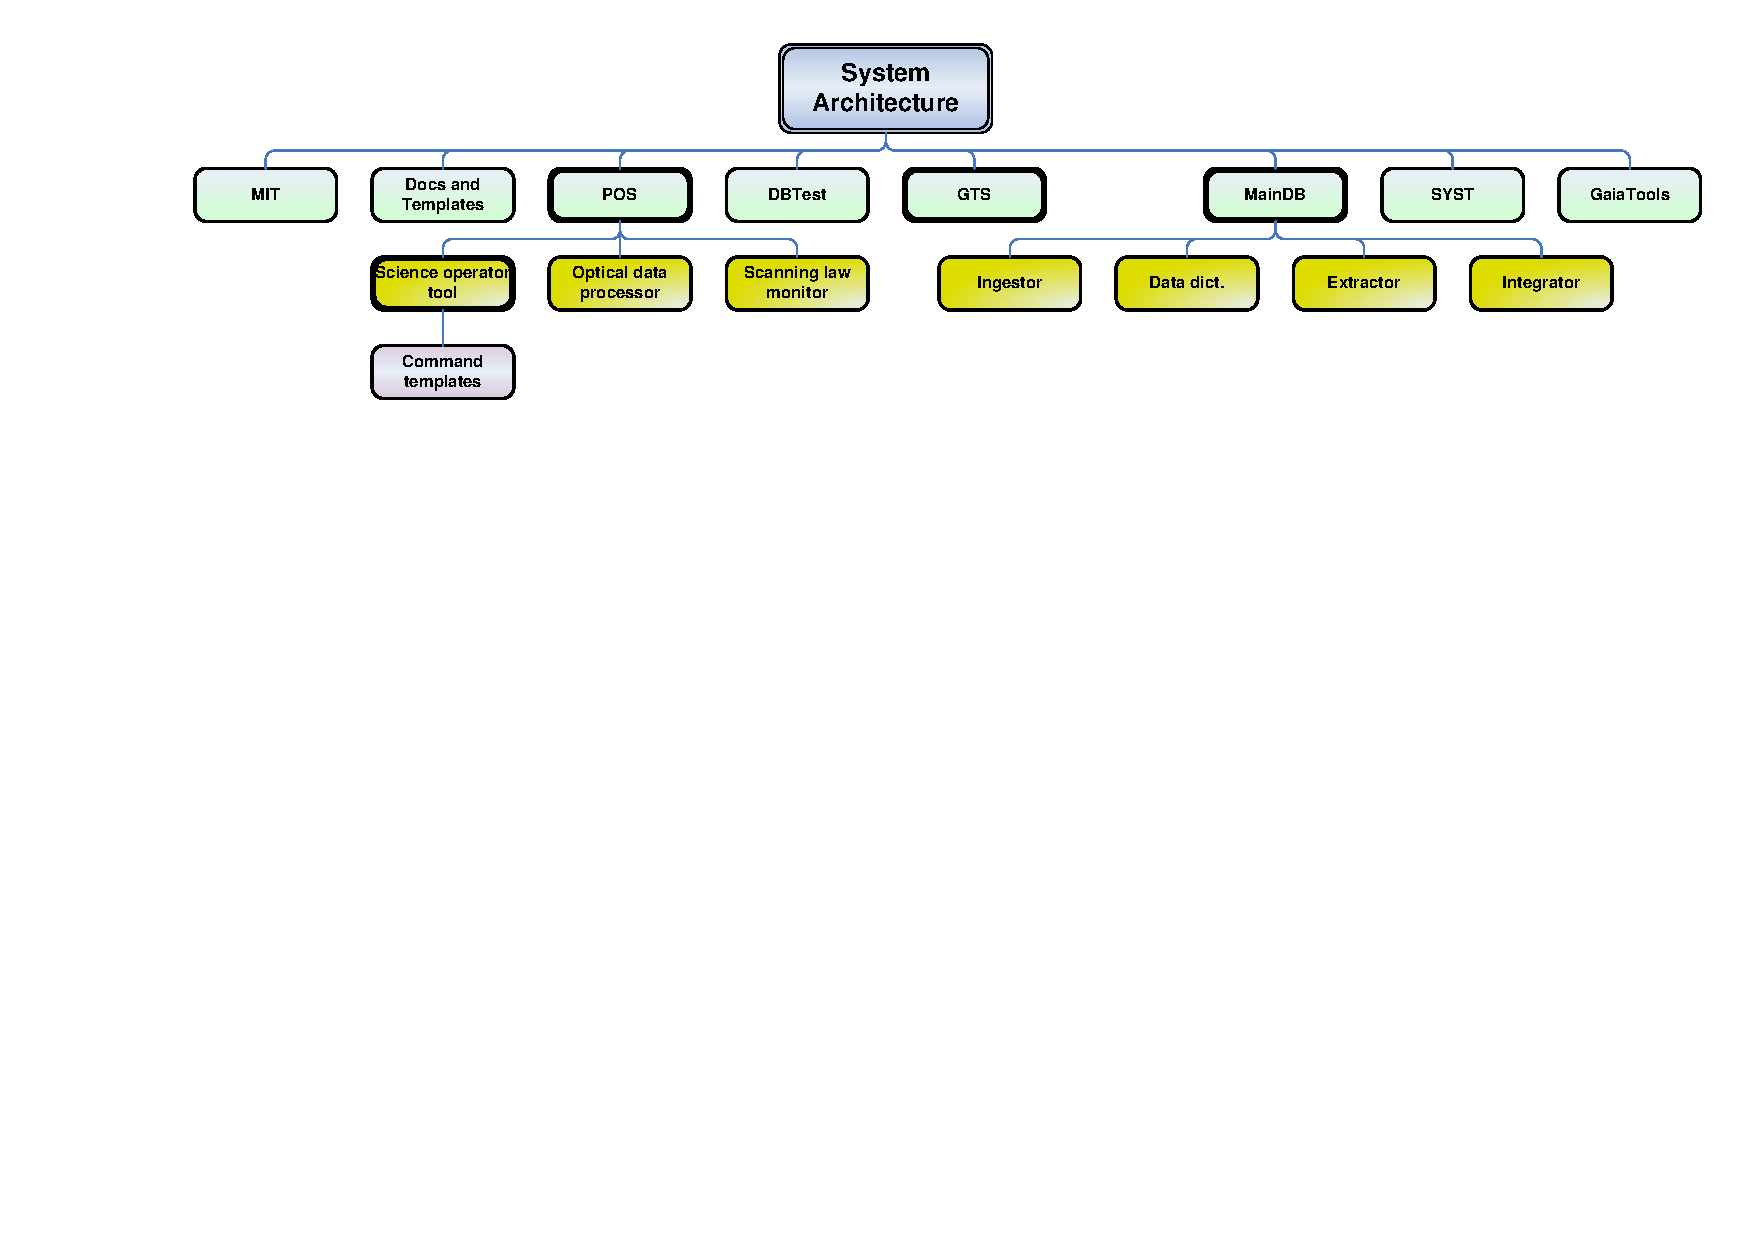
\includegraphics[scale=0.5,trim=0 12cm 0 0]{images/cu1Products}
\caption{Example Product tree a version of  CU1 product tree \label{fig:prod}}
\end{center}
\end{figure}


\subsection{Work Breakdown Structure and effort required}

In this section you should list the work packages and sub packages with the
the person responsible for each.  The effort required per year for each
workpackage is listed in \tabref{tab:CU1effort}.

If all WPS are in a directory called WPS the
script  GWPsummary.pl from the CU1/docs/common/scripts directory will
generate a table such as the one bellow which may be included.

Full details of all work packages are provided in \appref{sect:wpds}.
\scriptsize
\begin{longtable}{|l|p{0.5\textwidth}|p{0.2\textwidth}|}\hline
WP Number & Description & Manager \\\hline
 GWP-M-x01-00000 & Management and scientific coordination of CUx & CU-L\\\hline
\end{longtable}
\normalsize


The effortReq directory from the AO response is now in CU1/docs/common/effrotReq
the script for making the effort tables and sumaries from these files is now
in CU1/docs/common/scripts/effortTex.pl. You may use this script to generate a
table such as the one included bellow from CU1. To generate the table for your
CU or DPC you must set the environment variable DOCCOMMON to point to
CU1/docs/common. Preferably include DOCCOMON/scirpts in your path. Then run the script
passing your CUx as an argument i.e. for cu1
\begin{code}
effortTex.pl CU1
\end{code}

%Generated by c:\dpac\cu1\docs\common\scripts\effortTex.pl do not edit  - rather update .csv files in effortReq directory. 
\tiny \begin{longtable}{|l||r|r|r|r|r|r|r|r|r|r|r|r|r|r|}
\caption{\scriptsize Effort (staff months) required per work package for CU1. \label{tab:CU1effort}} 
 \\\hline
WP Number &2007 &2008 &2009 &2010 &2011 &2012 &2013 &2014 &2015 &2016 &2017 &2018 &2019 & {\bf Total} \\\hline
{\tt  \hfill  GWP-M-101}  & 9 &12 &12 &15 &12 &12 &11 &11 &11 &11 &14 &14 &12 &154 \\\hline
{\tt  \hfill  GWP-T-102}  & 14 &19 &17 &12 &7 &7 &6 &6 &6 &6 &5 &5 &5 &113 \\\hline
{\tt  \hfill  GWP-T-103}  & 20 &19 &21 &20 &20 &12 &10 &10 &10 &10 &18 &12 &4 &181 \\\hline
{\tt  \hfill  GWP-M-104}  & 4 &6 &6 &4 &4 &2 &2 &2 &2 &2 &1 &1 &1 &31 \\\hline
{\tt  \hfill  GWP-T-110}  & 9 &10 &11 &11 &11 &11 &8 &12 &12 &12 &8 &7 &7 &126 \\\hline
{\tt  \hfill  GWP-T-140}  & 10 &11 &7 &12 &7 &7 &0 &3 &0 &3 &4 &0 &0 &63 \\\hline
{\tt  \hfill  GWP-T-140}  & 30 &30 &30 &30 &30 &30 &0 &0 &0 &0 &0 &0 &0 &180 \\\hline
{\tt  \hfill  GWP-T-150}  & 1 &1 &1 &2 &3 &3 &0 &0 &0 &0 &0 &0 &0 &10 \\\hline
{\tt  \hfill  GWP-T-170}  & 0 &0 &0 &1 &1 &1 &1 &1 &1 &1 &0 &0 &0 &4 \\\hline
{\tt  \hfill  GWP-T-180}  & 27 &30 &31 &33 &32 &26 &16 &16 &15 &16 &24 &22 &22 &309 \\\hline
{\tt  \hfill  GWP-T-190}  & 21 &26 &16 &16 &24 &22 &1 &1 &1 &1 &1 &1 &1 &131 \\\hline
{\bf Total CU1 }&{\bf 142 } &{\bf 162 } &{\bf 151 } &{\bf 155 } &{\bf 150 } &{\bf 130 } &{\bf 52 } &{\bf 59 } &{\bf 56 } &{\bf 59 } &{\bf 74 } &{\bf 61 } &{\bf 51 } &{\bf 1300}\\\hline
\end{longtable} \normalsize


\section{Software management approach} \label{sect:managemntapp}
The management approach is heavily driven by the cyclical approach outlined
in \citell{LL:WOM-001} and defined in \citell{LL:RD-010}.

\subsection{Master schedule } \label{sect:mastschedule}

The global planning of the CU for the period 2006-2011.
General description of each cycle linking to the  milestones
listed in \secref{sect:milestones}.  Please also take note of the cycles
as listed with their reviews in \citell{LL:WOM-001}.

This should be high level and short giving an overview of important dates for the CU.

This document should be updated near the end of each cycle to
refine planning for the next cycle and reassess risks etc.

\subsection{Milestones}
Here list top-level milestones for the CU, including the final "end-to-end tests" of the CU data processing system. If there are only DU milestones then
one subsection for each DU to list the DU milestones for each cycle.

\subsubsection{Milestones for DUx \label{sect:milestones}}
A simple and short bullet list of clear objectives for each cycle.
This can be removed if all milestones are listed under the CU heading
i.e. then this list appears only once
\begin{itemize}
  \item Cycle 1
  \begin {itemize}
    \item Goal 1
  \end{itemize}
    \item Cycle 2
  \begin {itemize}
    \item Goal 1
   \end{itemize}
    \item Cycle 3
  \begin {itemize}
    \item Goal 1
  \end{itemize}
    \item Cycle 4
  \begin {itemize}
    \item Goal 1
  \end{itemize}
    \item Cycle 5
  \begin {itemize}
    \item Goal 1
  \end{itemize}
    \item Cycle 6
  \begin {itemize}
    \item Goal 1
  \end{itemize}
    \item Cycle 7
  \begin {itemize}
    \item Goal 1
  \end{itemize}
    \item Cycle 8
  \begin {itemize}
    \item Goal 1
  \end{itemize}
    \item Cycle 9
  \begin {itemize}
    \item Goal 1
  \end{itemize}
    \item Cycle 10
  \begin {itemize}
    \item Goal 1
  \end{itemize}
\end{itemize}

\subsection{Planning }
All cycles should be identified here, with formal DPAC reviews included.
Detail in the approaching cycle is in a later section.

The CU development plan should include top-level CU milestones to be achieved (from previous section), tasks that need to be done to reach these milestones, and critical deliveries from other CUs or ESA (when these need to be received).

If the CU has no DUs all planning may be in this section otherwise a
subsection such as \secref{sect:du1plan} should be added for each DU.

\subsubsection{ Planning for DUx \label{sect:du1plan}}
Here a gantt chart type planning is suggested linking this to the WBS and tasks.
This section is optional (see text above) and may be repeated for each DU.

\subsubsection{Deliverables\label{sect:deliverables}}
This section should list the deliveries that the CU must make to other CUs or ESA (\textit{not ESAC as DPC})

\begin{itemize}
    \item Critical delivery 1 (to CUx)
    \item Critical delivery 2 (to CUy)
\end{itemize}

\subsection{Assumptions, dependencies and constraints on \CU  \label{sect:assumptionsdep}}

\subsubsection{Assumptions  \label{sect:assumtions}}
The assumptions on which the plan is based.

\subsubsection{ Dependencies and constraints with respect to other CUs
\label{sect:cuconstraints}}

This section should list the critical deliverables (data, SW, etc.) that the CU must receive from other CUs, i.e. those items needed to stay on its development schedule.
\begin{itemize}
    \item Critical delivery 1 (from CUx)
    \item Critical delivery 2 (from CUy)
\end{itemize}

\subsubsection{Other dependencies and constraints  \label{sect:othercontraints}}

This section should list the critical deliveries that the CU must receive from outside DPAC, especially from ESA.
\begin{itemize}
    \item Critical delivery 1 (from ESA)
    \item Critical delivery 2 (from ESA)
\end{itemize}

\subsection{Risk Management \label{sect:riskmngt}}
Risk management is carried out in accordance with the DPAC risk management plan \citell{LL:RD-008}.

\subsubsection{Identification of Risks \label{sect:risks}}
Identification of technical, financial, human etc. risks at CU or DU / WP
level.
\newrisktype{DPAC-CUx} % probably just one per CU

\risk{Hardware prices}{5}{B}
% description
{It is possible hardware prices will not continue to drop. At todays prices the
CU1 hardware will cost far more than budgeted.}
%Mitigation
{Try to have money put in contingency for hardware.}

% copy above 'risk' to add more - numbers added automatically.


\subsubsection{Actions related to risk management  \label{sect:riskactions}}
The actions taken at CU, organizational, DPAC, etc. level to manage identified risks.

\subsection{Monitoring mechanisms  \label{sect:monitoring}}
The monitoring mechanisms for managing the work (e.g. progress report,
progress meeting, action item lists).

\subsection{Training plan  \label{sect:Training Plan}}
Identification of missing skills and training needs.

\section{Software development  approach \label{sect:approach}}
Could be a link to \citell{LL:WOM-001}.

\subsection{\CU ~software development strategy \label{sect:strategy}}
CU development strategy elements (not covered by \citell{LL:TL-001}).

\subsection{Detailed description of \CU ~cycle Z \label{sect:detailcyclez}}
Review of objectives, activities, input, output, completion criteria, internal reviews, etc. of the cycle Z. The development schedule (plan) for the upcoming cycle.

One of these for each cycle more detail in the upcoming one (i.e. replace "Z" with a cycle number).

\subsection{Internal reviews and associated documentation
\label{sect:internalreview}}
Description of the scope and purpose of each identified internal review, relevant deliverables and expected
outputs. The role of involved parties at each internal review shall be
described here. Formalities are outlined in the QA document.

\section{Software Configuration Management \label{sect:configmngt}}
Detailed description of the software configuration management process, activities and procedures (including
software problem report, change request management are covered in
\citell{LL:WOM-012} configuration management plan.

Practical information on implementing configuration management is contained in
the Engineering Guide \citell{LL:WOM-011}.

In this section the configuration control board organisation,
configuration items etc are listed for \CU.

\subsection{Configuration Item List and Baseline \label{sect:cis}}
This is a list of the configuration items for \CU.
%For each item fill a row in the table
\begin{longtable} {|p{0.2\textwidth}|p{0.2\textwidth}|p{0.2\textwidth}|p{0.25\textwidth}|}\hline
{\bf Prod. Name} & {\bf WP Number}& {\bf Manager} &{\bf SRS}  \\\hline
As outlined in SRS Template a name e.g \newline AGIS &
Full WP Number e.g \newline {\scriptsize GWP-T-320-10000}  &
Name of manager  &
{\scriptsize GAIA-C3-SP-ESAC-UL-019-1 \citell{LL:UL-019}} \\\hline
\end{longtable}

{\bf Note:} the SRS document code includes the issue number effectively this is
the  configuration baseline.
%note keep this note in your document.

\subsection{Configuration Control Board}
Describe the Configuration Control Board organisation and members.
Guidelines for the setting up the the \CU CCB are in \citell{LL:WOM-012}.

Here actual names of the members should be listed and proposed frequency of meetings.

\section{\CU ~Specific  Policies
\label{sect:epcifictech}}
Any deviations from the product assurance plan should be listed here.
Also any specific engineering techniques not covered in the engineering guide
should be mentioned.
Any configuration management deviating or on top of the SCMP should be listed.

This section is optional and may be dropped if the CU adheres to the PA and CM
plans.

\appendix

\section{Product assurance compliance Matrix \label{sect:compmat}}
A table will be provided for this section when the QA plan id

\section {Detail Work Package Descriptions for \CU \label{sect:wpds}}
List here the detailed work package descriptions using the \code{gwp}
environment. Typically there would be a file for each WP usually named
with the WP number. The template example is included here :

%
%	Template file Gaia WP description
%
%	Author: U. Lammers, Mon Nov 14 18:47:05 CET 2005
%
%	$Id: gwptemplate.tex 14339 2007-02-07 16:32:27Z womullan $
%

%
%	Start description of WP
%	Environment: \GWP
%	Arguments:
%		1) WP code adhering to GAIA-C1-TN-ESAC-WOM-001
%		2) Title
%
\begin{GWP}{T-CNNN-PPPP}{Work Package Title}
%
%	Specify provider and manager of WP
%	Command: \gwpprovmanag
%	Argument(s):
%		1) Provider: list of individuals performing the work (free text)
%		2) Manager:	WP manager's name and name of deputy where appropriate
%			(free text)
%
\gwpprovmanag{List of people doing the work}{Name of WP's manager}
%
%	Define start+end of WP plus total man power effort
%	Command: \gwpstartendeffort
%	Argument(s):
%		1) Start of WP [dd/mm/yyyy]
%		2) End of WP [dd/mm/yyyy]
%		3) The approximate total effort allocated or estimated for the
%		   package [man months] (number without unit)
%
\gwpstartendeffort{dd/mm/yyyy}{dd/mm/yyyy}{nnn}

%	Descripiton of objective of WP
%	Command: \gwpobjective
%	Argument(s):
%		1) Description (free text)
%
\gwpobjective{Describe here the objective of the WP - this is a free
text input - all \LaTeX\ constructs can be used (lists, verbatim, etc.)}
%
%	List all tasks this WP consists of
%	Command: \gwptask
%	Argument(s):
%		1) Task list (free text)
\gwptask{Listing of all tasks this WP consists of - this is a free text
text input - all \LaTeX\ constructs can be used, e.g.\
\begin{enumerate}
\item Task 1
\begin{enumerate}
\item SubTask 1
\end{enumerate}
\item Task 2
\item Task 3
\end{enumerate}
}
%
%	Specify input and output of this WP
%	Commands: \gwpinput + \gwpoutput
%	Argument(s):
%		1) List of WP inputs/outputs (free text)
%
\gwpinput{List here all inputs to the WP}
\gwpoutput{List here all outputs of the WP}
%
%	Specifiy WP deliverables
%	Command: \gwpdeliver
%	Argument(s):
%		1) List of WP deliverables, e.g. software or report under configuration
%		   control
%		
\gwpdeliver{List of WP deliverables, e.g. software or report under
configuration control}
%
%	Specify WP dependencies
%	Command: \gwpdepend
%	Argument(s):
%		1) List of dependencies of this WP (free text)
%
\gwpdepend{List of all dependencies of this WP}
%
%	Specify all interfaces of this WP
%	Command: \gwpinterface
%	Argument(s):
%		1) List of all interfaces of this WP, i.e. links with other
%		   tasks, WPs, or CUs (free text)
%
\gwpinterface{List of all interfaces of this WP, i.e.\ links with other
tasks, WPs, or CUs}
%
%	Specify remarks
%	Command: \gwpremark
%	Argument(s):
%		1) Remarks (free text)
%
\gwpremark{Remarks - free text}
%
%	END of GWP enviroment
%
\end{GWP}


This entire section may be generated from a directory full of GWP files
using GWPsummary.pl from the CU1/docs/common/scripts directory.


\end{document}
